\chapter{Neclear Physics}
\begin{enumerate}
	\item  What should be the minimum energy of a photon for it split an alpha particle at rest into a tritium and a proton?
	(The masses of ${ }_2^4 \mathrm{He},{ }_1^3 \mathrm{H}$ and ${ }_1^1 \mathrm{H}$ are $4.0026 \mathrm{amu}, 3 \cdot 0161 \mathrm{amu}$ and $1.0073 \mathrm{amu}$ respectively, and $1 \mathrm{amu} \approx 938 \mathrm{MeV})$
	 \begin{tasks}(2)
		\task[\textbf{a.}] $32 \cdot 2 \mathrm{MeV}$
		\task[\textbf{b.}]$3 \mathrm{MeV}$
		\task[\textbf{c.}]$19 \cdot 3 \mathrm{MeV}$
		\task[\textbf{d.}] $931.5 \mathrm{MeV}$
	\end{tasks}
\begin{answer}
	$$
	\begin{aligned}
	{ }_2 H e^4&+\gamma \rightarrow{ }_1 H^3+{ }_1 H^1\\
	E_{p h}^{\min }&=Q=\left[M_{{ }_2 H^4}-M_{{ }_1 H^3}-M_{{ }_1 H^1}\right] \times 938 \mathrm{MeV}\\
	&=[4 \cdot 0026-3 \cdot 0161-1 \cdot 0073] \times 938 \\
	&=-19 \cdot 5 \mathrm{MeV}
\end{aligned}
$$
So the correct answer is \textbf{Option (c)}
\end{answer}
	\item  A particular radioisotope has a half life of 5 days. What is the probability of decay (in percentage) in 15 days?
	 \begin{tasks}(2)
		\task[\textbf{a.}]$87 \cdot 5$
		\task[\textbf{b.}]75
		\task[\textbf{c.}] $25 \cdot 5$
		\task[\textbf{d.}] $13 \cdot 5$
	\end{tasks}
\begin{answer}
	$$
	\begin{aligned}
	P&=\frac{N_0-N_0(1 / 2)^{15 / 5}}{N_0}=\frac{N_0-\frac{N_0}{8}}{N_0} \times 100\\
	P&=87 \cdot 5 \%
\end{aligned}
$$
So the correct answer is \textbf{Option (a)}
\end{answer}
	\item  The intrinsic electric dipole moment of a nucleus ${ }_Z^A X$
	 \begin{tasks}(2)
		\task[\textbf{a.}]Increases with $Z$, but independent of $A$
		\task[\textbf{b.}]Decreases with $Z$, but independent of $A$
		\task[\textbf{c.}]Is always zero
		\task[\textbf{d.}]Increases with $Z$ and $A$
	\end{tasks}
\begin{answer}
	So the correct answer is \textbf{Option (c)}
\end{answer}
	\item  Parity and spin of ${ }_6 C^{12}$ nuclei is
	 \begin{tasks}(2)
		\task[\textbf{a.}]Odd, zero
		\task[\textbf{b.}]Odd, $\frac{1}{2}$
		\task[\textbf{c.}]Even, zero
		\task[\textbf{d.}]Even, $\frac{1}{2}$ 
	\end{tasks}
\begin{answer}
	$$
	\begin{aligned}
\text { For even } N \text {, even } Z \text { nuclei spin will be zero and parity will be even. }
	\end{aligned}
	$$
	So the correct answer is \textbf{Option (c)}
\end{answer}
	\item  If in a spontaneous $\alpha$ - decay of neutron ${ }_{92}^{232} U$ at rest, the total energy released in the reaction is $Q$, then the energy carried by the $\alpha$-particle is
	 \begin{tasks}(2)
		\task[\textbf{a.}] $57 Q / 58$
		\task[\textbf{b.}]$Q / 57$
		\task[\textbf{c.}]$Q / 58$
		\task[\textbf{d.}]$23 Q / 58$ 
	\end{tasks}
\begin{answer}
	$$
	\begin{aligned}
	Q_\alpha&=K_\alpha \frac{A}{A-4}\\
	Q&=K_\alpha \frac{232}{232-4} \\
	K_\alpha&=\frac{238}{232} Q=\frac{57 Q}{58}
\end{aligned}
$$
So the correct answer is \textbf{Option (a)}
\end{answer}
	\item  The spin-parity assignments for the ground and first excited states of the isotope ${ }_{28}^{57} \mathrm{Ni}$, in the single particle shell model, are
	 \begin{tasks}(2)
		\task[\textbf{a.}]$\frac{1}{2}^{-}$and $\frac{3}{2}^{-}$
		\task[\textbf{b.}]$\frac{5}{2}^{+}$and $\frac{7^{+}}{2}$
		\task[\textbf{c.}]$\frac{3}{2}^{+}$and $\frac{5}{2}^{+}$
		\task[\textbf{d.}]$\frac{3^{-}}{2}$ and $\frac{5^{-}}{2}$
	\end{tasks}
\begin{answer}
	$$
	\begin{aligned}
	{ }_{28}^{57} N i \rightarrow N&=29:\left.\left.\left.\quad 1 s_{1 / 2}^2\right|^2 1 p_{3 / 2}^4 1 p_{1 / 2}^2\right|^8 1 d_{5 / 2}^6 2 s_{1 / 2}^2 1 d_{3 / 2}^4\right|^{20} 1 f_{7 / 2}^8 2 p_{3 / 2}^1 1 f_{5 / 2}^0\\
	G S \rightarrow J^\pi&=\frac{3^{-}}{2} \qquad \text { as } \pi=(-1)^1=-v e\\
\text { First excited state}&\text{ will be corresponding to the following transition of unpaired neutron }\\
2 p_{3 / 2}^0 &\longrightarrow 1 f_{5 / 2}^1\\
\text{First excited state}\\
J^\pi&=\frac{5^{-}}{2} \quad \text { as } \pi=(-1)^3=-v e
\end{aligned}
$$
So the correct answer is \textbf{Option (d)}
\end{answer}
	\item  A nucleus decays by the emission of a gamma ray from an exited state of spin parity $2^{+}$ to the ground state $O^{+}$. What is the type of the corresponding radiation?
	 \begin{tasks}(2)
		\task[\textbf{a.}] Magnetic dipole.
		\task[\textbf{b.}]Electric quadrupole.
		\task[\textbf{c.}]Electric dipole.
		\task[\textbf{d.}] Magnetic quadrupole
	\end{tasks}
\begin{answer}
	$$
	\begin{aligned}
	J_1&=1, J_2=0\\
	J&=\left|J_1-J_2\right|-\left(J_1+J_2\right) \\
	J&=2\\
	\text{Parity change }&=\text{ No}\\
\text{	Thus, the corresponding }&\text{radiation is electric quadrupole type.}
\end{aligned}
$$
So the correct answer is \textbf{Option (b)}
\end{answer}
	\item The radius of a ${ }_{29}^{64} \mathrm{Cu}$ nucleus is measured to be $4 \cdot 8 \times 10^{-13} \mathrm{~cm}$. The radius of a ${ }_{12}^{27} \mathrm{Mg}$ nucleus can be estimated to be
	 \begin{tasks}(2)
		\task[\textbf{a.}]$2 \cdot 86 \times 10^{-13} \mathrm{~cm}$
		\task[\textbf{b.}] $5 \cdot 2 \times 10^{-13} \mathrm{~cm}$
		\task[\textbf{c.}] $3 \cdot 6 \times 10^{-13} \mathrm{~cm}$
		\task[\textbf{d.}] $8 \cdot 6 \times 10^{-13} \mathrm{~cm}$
	\end{tasks}
\begin{answer}
	$$
	\begin{aligned}
 R_{M g}&=R_{C u}\left(\frac{A_{M g}}{A_{C u}}\right)^{1 / 3}=4 \cdot 8 \times 10^{-13} \times\left(\frac{27}{64}\right)^{1 / 3}\\
	&=3 \cdot 6 \times 10^{-13} \mathrm{~cm}
\end{aligned}
$$
So the correct answer is \textbf{Option (c)}
\end{answer}
	\item The ground state of the deuteron is a
	 \begin{tasks}(2)
		\task[\textbf{a.}]Pure ${ }^3 S_1$ state
		\task[\textbf{b.}]Pure ${ }^3 P_1$ state
		\task[\textbf{c.}] Pure ${ }^3 S_1$ and ${ }^3 P_1$ states
		\task[\textbf{d.}] Mixture of ${ }^3 S_1$ and ${ }^3 D_1$ states
	\end{tasks}
\begin{answer}
So the correct answer is \textbf{Option (d)}
\end{answer}
	\item The neutron and proton form a deuteron bound state which is stable while there is no bound state for two neutrons because?
	 \begin{tasks}(2)
		\task[\textbf{a.}]Nuclear forces are saturated
		\task[\textbf{b.}]Nuclear forces are spin dependent
		\task[\textbf{c.}]Nuclear forces are charge independent
		\task[\textbf{d.}] Nuclear forces depends upon magnetic moment
	\end{tasks}
\begin{answer}
	$$
	\begin{aligned}
	&\text{ The energy of the singlet state is higher than the triplet state. A combination of proton }\\
	&\text{and neutron form triplet state while combination of neutron-neutron forms singlet state,}\\
	&\text{ which is higher in energy and no bound state is possible. This is confirming the spin }\\
	&\text{dependency of the nuclear state.}
\end{aligned}
$$
So the correct answer is \textbf{Option (b)}
\end{answer}
	\item A heavy nucleus is found to contain more neutrons than protons. This fact is related to which one of the following statements:
	 \begin{tasks}(2)
		\task[\textbf{a.}]The nuclear force between neutrons is stronger than that between protons.
		\task[\textbf{b.}]The nuclear force between protons, so that a range than those between neutrons, so that a smaller number of protons are held together by the nuclear force.
		\task[\textbf{c.}] Protons are unstable, so their number in a nucleus diminishes.
		\task[\textbf{d.}]  It costs more energy to add a proton to a (heavy) nucleus than a neutron because of the coulomb repulsion between protons.
	\end{tasks}
\begin{answer}
So the correct answer is \textbf{Option (d)}
\end{answer}
	\item Under parity operation the following does not change sign.
	 \begin{tasks}(2)
		\task[\textbf{a.}]Momentum
		\task[\textbf{b.}] Electric field
		\task[\textbf{c.}] Magnetic field
		\task[\textbf{d.}]  Spin
	\end{tasks}
\begin{answer}
	So the correct answer is \textbf{Option (d)}
\end{answer}
	\item Under time reversal operation the following does not change sign.
	 \begin{tasks}(2)
		\task[\textbf{a.}]Momentum
		\task[\textbf{b.}] Electric field
		\task[\textbf{c.}] Magnetic field
		\task[\textbf{d.}] Spin
	\end{tasks}
\begin{answer}
	So the correct answer is \textbf{Option (b)}
\end{answer}
	\item Is nature invariant under the combined parity and charge conjugation operation?
	 \begin{tasks}(2)
		\task[\textbf{a.}]Yes
		\task[\textbf{b.}]No
		\task[\textbf{c.}]Depend on the process
		\task[\textbf{d.}] None of these
	\end{tasks}
\begin{answer}
	So the correct answer is \textbf{Option (b)}
\end{answer}
	\item In deep inelastic scattering electrons are scattered off protons to determine if a proton has any internal structure. The energy of the electron for this must be at least
	 \begin{tasks}(2)
		\task[\textbf{a.}] $1.25 \times 10^9 \mathrm{eV}$
		\task[\textbf{b.}]$1.25 \times 10^{12} \mathrm{eV}$
		\task[\textbf{c.}]$1.25 \times 10^6 \mathrm{eV}$
		\task[\textbf{d.}]  $1.25 \times 10^8 \mathrm{eV}$
	\end{tasks}
\begin{answer}
	$$
	\begin{aligned}
\text{The internal structure of proton can}&\text{ only be determined if the wavelength of the }\\
\text{incoming electron is nearly equal to}&\text{  the size of the proton}\\
	i.e. \lambda&=R=1.2 A^{1 / 3}(\mathrm{fm})=1.2 \mathrm{fm}=1.2 \times 10^{-15} \mathrm{~m}\\
\text{	According to de-Broglie relation,} \lambda&=\frac{h}{p}=\frac{h}{\sqrt{2 m E}}\\
	\text{This can be also written as }E^2&=h^2 \lambda^2 / c^2+m_0^2 c^4
\end{aligned}
$$
	So the correct answer is \textbf{Option (b)}
\end{answer}
	\item The root-mean-square (r.m.s) energy of a nucleon in a nucleus of atomic number $A$ in its ground state varies as:
	 \begin{tasks}(2)
		\task[\textbf{a.}] $A^{4 / 3}$
		\task[\textbf{b.}]$A^{1 / 3}$
		\task[\textbf{c.}]$A^{-1 / 3}$
		\task[\textbf{d.}] $A^{-2 / 3}$
	\end{tasks}
\begin{answer}
	So the correct answer is \textbf{Option (c)}
\end{answer}
	\item Let $E_S$ denotes the contribution of the surface energy per nucleon in the liquid drop model. The ratio $E_S\left({ }_{13}^{27} \mathrm{Al}\right): E_S\left({ }_{30}^{64} \mathrm{Zn}\right)$ is
	 \begin{tasks}(2)
		\task[\textbf{a.}]$2: 3$
		\task[\textbf{b.}] $4: 3$
		\task[\textbf{c.}]$5: 3$
		\task[\textbf{d.}]  $3: 2$
	\end{tasks}
\begin{answer}
	$$
	\begin{aligned}
	E_S&=\frac{B}{A}=\frac{A^{\frac{2}{3}}}{A} \propto A^{-\frac{1}{3}} \Rightarrow \frac{E_S(A l)}{E_S\left(Z_n\right)}=\frac{(27)^{-\frac{1}{3}}}{(64)^{-\frac{1}{3}}}=\frac{(64)^{\frac{1}{3}}}{(27)^{\frac{1}{3}}}=\frac{4}{3}
\end{aligned}
$$
	So the correct answer is \textbf{Option (b)}
\end{answer}
	\item The binding energy of a light nucleus $(Z, A)$ in $\mathrm{MeV}$ is given by the approximate formula
	$$
	B(A, Z) \approx 16 A-20 A^{2 / 3}-\frac{3}{4} Z^2 A^{-1 / 3}+30 \frac{(N-Z)^2}{A}
	$$
	where $N=A-Z$ is the neutron number. The value of $Z$ of the most stable isobar for a given $A$ is
	 \begin{tasks}(2)
		\task[\textbf{a.}]$\frac{A}{2}\left(1-\frac{A^{2 / 3}}{160}\right)^{-1}$
		\task[\textbf{b.}]$\frac{A}{2}$
		\task[\textbf{c.}] $\frac{A}{2}\left(1-\frac{A^{2 / 3}}{120}\right)^{-1}$
		\task[\textbf{d.}] $\frac{A}{2}\left(1+\frac{A^{4 / 3}}{64}\right)^{-1}$
	\end{tasks}
\begin{answer}
	$$
	\begin{aligned}
	\left.\frac{\partial B}{\partial Z}\right|_{Z=Z^{\prime}}&=0 \Rightarrow Z^{\prime}=\frac{A}{2}\left(1-\frac{A^{2 / 3}}{160}\right)^{-1}
	\end{aligned}
	$$
		So the correct answer is \textbf{Option (a)}
\end{answer}
	\item If the binding energy $B$ of a nucleus (mass number $A$ and charge $Z$ ) is given by
	$$
	B=a_V A-a_S A^{2 / 3}-a_{s y m} \frac{(2 Z-A)^2}{A}+\frac{a_C Z^2}{A^{1 / 3}}
	$$
	where $a_V=16 \mathrm{MeV}, a_S=16 \mathrm{MeV}, a_{s y m}=24 \mathrm{MeV}$ and $a_C=0.75 \mathrm{MeV}$, then for the most stable isobar for a nucleus with $A=216$ is
	 \begin{tasks}(2)
		\task[\textbf{a.}]68
		\task[\textbf{b.}]72
		\task[\textbf{c.}]84
		\task[\textbf{d.}] 92
	\end{tasks}
\begin{answer}
	$$
	\begin{aligned}
	\text { For the most stable isobar for a nucleus } \frac{d B}{d Z}&=0 \Rightarrow-a_{s y m} \frac{2(2 Z-A) \times 2}{A}+\frac{2 a_C Z}{A^{1 / 3}}=0\\
	\Rightarrow 24 \frac{2(2 Z-216) \times 2}{216}+0.75 \frac{2 Z}{(216)^{1 / 3}}&=0 \Rightarrow \frac{4(2 Z-216)}{9}+\frac{3}{4} \frac{2 Z}{6}=0\\
	\Rightarrow \frac{4(2 Z-216)}{9}+\frac{Z}{4}=0 \Rightarrow 16(2 Z-216)+9 Z&=0 \Rightarrow 41 Z=216 \times 16 \Rightarrow Z=82.3
\end{aligned}
$$
	So the correct answer is \textbf{Option (c)}
\end{answer}
	\item Of the nuclei of mass number $A=125$, the binding energy calculated from the liquid drop model (given that the coefficients for the Coulomb and the asymmetry energy are $a_c=0.7 \mathrm{MeV}$ and $a_{s y m}=22.5 \mathrm{MeV}$ respectively) is a maximum for
	 \begin{tasks}(2)
		\task[\textbf{a.}]${ }_{54}^{125} \mathrm{Xe}$
		\task[\textbf{b.}]${ }_{53}^{124} I$
		\task[\textbf{c.}]${ }_{52}^{125} \mathrm{Te}$
		\task[\textbf{d.}] ${ }_{51}^{125} \mathrm{Sb}$
	\end{tasks}
\begin{answer}
	$$
	\begin{aligned}
	Z_0&=\frac{4 a_a+a_c A^{-1 / 3}}{2 a_c A^{-1 / 3}+8 a_a A^{-1}}=\frac{4 a_a A+a_c A^{2 / 3}}{8 a_a+2 a_c A^{2 / 3}} \Rightarrow Z_0=\frac{4 \times 22.5 \times 125+0.7\left(5^3\right)^{2 / 3}}{8 \times 22.5+2 \times 0.7\left(5^3\right)^{2 / 3}}\\
	\Rightarrow Z_0&=\frac{11250+17.5}{180+35}=\frac{11267.5}{215}=52.4 \Rightarrow Z_0 \approx 52
\end{aligned}
$$
	So the correct answer is \textbf{Option (c)}
\end{answer}
	\item A radioactive element $X$ decays to $Y$, which in turn decays to a stable elements $Z$. The decay constant from $X$ to $Y$ is $\lambda$, and that from $Y$ to $Z$ is $\lambda_2$. If to begin with, there are only $N_0$ atoms of $X$, at short times $\left(t<<1 / \lambda_1\right.$ as well as $\left.1 / \lambda_2\right)$ the number of atoms of $Z$ will be
 \begin{tasks}(2)
	\task[\textbf{a.}]$\frac{1}{2} \lambda_1 \lambda_2 N_0 t^2$
	\task[\textbf{b.}] $\frac{\lambda_1 \lambda_2}{2\left(\lambda_1+\lambda_2\right)} N_0 t$
	\task[\textbf{c.}]$\left(\lambda_1+\lambda_2\right)^2 N_0 t^2$
	\task[\textbf{d.}] $\left(\lambda_1+\lambda_2\right) N_0 t$
\end{tasks}
\begin{answer}
	$$
	\begin{aligned}
	N_1&=N_0 e^{-\lambda_1 t}=N_0\left[1-\lambda_1 t+\frac{\lambda_1{ }^2 t^2}{2}\right]\\
	N_2&=\frac{N_0 \lambda_1}{\lambda_2-\lambda_1}\left[e^{-\lambda_1 t}-e^{-\lambda_2 t}\right] \\
	&=\frac{N_0 \lambda_1}{\lambda_2-\lambda_1}\left[1-\lambda_1 t+\frac{\lambda_1^2 t^2}{2}-1+\lambda_2 t-\frac{\lambda_2^2 t^2}{2}\right] \\
	&=\frac{N_0 \lambda_1}{\lambda_2-\lambda_1}\left[\left(\lambda_2-\lambda_1\right) t-\frac{\left(\lambda_2^2-\lambda_1^2\right) t^2}{2}\right]=N_0 \lambda_1\left[t-\frac{\left(\lambda_2-\lambda_1\right)}{2} t^2\right] \\
	&=N_0 \lambda_1 t-\frac{N_0}{2} \lambda_1\left(\lambda_2+\lambda_2\right) t^2\\
	N_3&=N_0-N_1-N_2 \\
	N_3&=\frac{1}{2} \lambda_1 \lambda_2 N_0 t^2
\end{aligned}
$$
	So the correct answer is \textbf{Option (a)}
\end{answer}
	\item The ground state of ${ }_{82}^{207} \mathrm{~Pb}$ nucleus has spin-parity $J^P=\frac{1^{-}}{2}$, while the first exited state has $J^P=\frac{5^{-}}{2}$. The electromagnetic radiation emitted when the nucleus makes a transition from the first exited state to ground state are
 \begin{tasks}(2)
	\task[\textbf{a.}]$E_2$ or $E_3$
	\task[\textbf{b.}] $M_2$ or $E_3$
	\task[\textbf{c.}]$E_2$ or $M_3$
	\task[\textbf{d.}] $M_2$ or $M_3$	
\end{tasks}
\begin{answer}
	$$
	\begin{aligned}
	J_i&=\frac{1}{2}, J_f=\frac{5}{2}, \quad \Delta \pi=\mathrm{No}\\
	J&=\left|J_2-J_f\right| \cdots .\left(J_i+J_f\right) \\
	J&=2\ ,\ 3\\
&	\ E 2 M 3
\end{aligned}
$$
	So the correct answer is \textbf{Option (c)}
\end{answer}
	\item The threshold temperature above which the thermonuclear reaction
$$
{ }_2^3 \mathrm{He}+{ }_2^3 \mathrm{He} \rightarrow{ }_2^4 \mathrm{He}+2{ }_1^1 \mathrm{H}+12 \cdot 86 \mathrm{MeV}
$$
Can occur is (use $e^2 / 4 \pi \epsilon_0=1.44 \times 10^{-15} \mathrm{MeV}-m$ )
 \begin{tasks}(2)
	\task[\textbf{a.}]$1.28 \times 10^{10} \mathrm{~K}$
	\task[\textbf{b.}]$1.28 \times 10^9 \mathrm{~K}$
	\task[\textbf{c.}] $1.28 \times 10^8 \mathrm{~K}$
	\task[\textbf{d.}] $1.28 \times 10^7 \mathrm{~K}$
\end{tasks}
\begin{answer}
	$$
	\begin{aligned}
	\frac{3}{2} K_B T&=\frac{1}{4 \pi \epsilon_0} \frac{(+2 e)(+2 e)}{2 R_0\left(A^{1 / 3}\right)} \qquad \because r=2 R\\
	\frac{3}{2} \times 1.38 \times 10^{-23} T &=\frac{e^2}{4 \pi \epsilon_0} \frac{4}{2 \times(1 \cdot 2 f m) \times(3)^{1 / 3}} \\
	&= \frac{(1 \cdot 44 \mathrm{MeV}-\mathrm{fm})}{2 \times(1 \cdot 2 \mathrm{fm}) \times 1.44}\\
	\frac{3}{2} \times 1 \cdot 38 \times 10^{-23} T &=\frac{\left(1 \cdot 44 \times 1 \cdot 6 \times 120^{-13} J\right) \times 4}{2 \times 1 \cdot 2 \times 1.44} \\
	T &=\frac{1 \cdot 6 \times 4 \times 2}{3 \times 2 \times 1 \cdot 2 \times 1.38} \times 10^{10} \mathrm{~K} \\
	T &=1 \cdot 28 \times 10^{10} \mathrm{~K}
\end{aligned}
$$
So the correct answer is \textbf{Option (a)}
\end{answer}
	\item The first excited state of the rotational $45 \mathrm{keV}$ above the ground state. The energy of second excited state (in $\mathrm{keV}$ ) is
 \begin{tasks}(2)
	\task[\textbf{a.}]150
	\task[\textbf{b.}]120
	\task[\textbf{c.}]90
	\task[\textbf{d.}] 60
\end{tasks}
\begin{answer}
	$$
	\begin{aligned}
	E_J&=\frac{\hbar^2}{2 I} J(J+1) \\
	\frac{E_2}{E_1}&=\frac{4(4+1)}{2(2+1)}=\frac{10}{3} \\
	E_2=\frac{10}{3} \times 45&=150 \mathrm{keV}
\end{aligned}
$$
So the correct answer is \textbf{Option (a)}
\end{answer}
	\item A permanently deformed even-even nucleus with $J^P=2^{+}$rotational energy $93 \mathrm{keV}$. The energy of the next excited state is
 \begin{tasks}(2)
	\task[\textbf{a.}] $372 \mathrm{keV}$
	\task[\textbf{b.}]$310 \mathrm{keV}$
	\task[\textbf{c.}] $273 \mathrm{keV}$
	\task[\textbf{d.}] $186 \mathrm{keV}$
\end{tasks}
\begin{answer}
	$$
	\begin{aligned}
	\frac{E_{4^{+}}}{E_{2^{+}}}&=\frac{4(4+1)}{2(2+1)}\\
	E_{4^{+}}&=\frac{10}{3} \times E_{2^{+}}=\frac{10}{3} \times 93 \mathrm{keV} \\
	E_{4^{+}}&=310 \mathrm{keV}
\end{aligned}
$$
So the correct answer is \textbf{Option (b)}
\end{answer}
	\item The difference in the coulomb energy between the mirror nuclei ${ }_{24}^{49} \mathrm{Cr}$ and ${ }_{25}^{49} \mathrm{Mn}$ is $6 \cdot 0 \mathrm{MeV}$. Assume that the nuclei have a spherically symmetric charge distribution and that $e^2 /\left(4 \pi \epsilon_0\right)$ is approximately $1 \cdot 0 \mathrm{MeV}-f m$, the radius of the ${ }_{25}^{49} \mathrm{Mn}$ is
  \begin{tasks}(2)
 	\task[\textbf{a.}] $4.9 \times 10^{-13} \mathrm{~m}$
 	\task[\textbf{b.}]$4.9 \times 10^{-15} \mathrm{~m}$
 	\task[\textbf{c.}]$5 \cdot 1 \times 10^{-13} \mathrm{~m}$
 	\task[\textbf{d.}] $5 \cdot 1 \times 10^{-15} \mathrm{~m}$	
 \end{tasks}
\begin{answer}
	$$
	\begin{aligned}
	\Delta E&=\frac{e^2}{4 \pi \epsilon_0} \frac{3\left(Z_1^2-Z_2^2\right)}{5 R}\\
	6 \mathrm{MeV}&=1 \cdot 0(\mathrm{MeV}-f m) \frac{3 \times\left(25^2-24^2\right)}{5 R}\\
	R&=\frac{3 \times 49}{6 \times 5}=4.9 \mathrm{fm}
\end{aligned}
$$
So the correct answer is \textbf{Option (b)}
\end{answer}
\item  The low lying energy levels due to the vibrational excitations of an even-even nucleus are shown in figure below:
\begin{figure}[H]
	\centering
	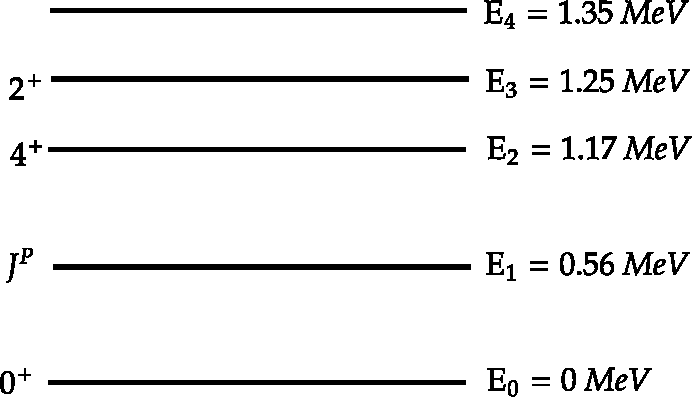
\includegraphics[height=3.5cm,width=6.2cm]{NP-1}
\end{figure}
	The spin-parity $J^P$ of the level $E_1$ is
	 \begin{tasks}(2)
		\task[\textbf{a.}]$1^{+}$
		\task[\textbf{b.}]$1^{-}$
		\task[\textbf{c.}]$2^{-}$
		\task[\textbf{d.}]$2^{+}$
	\end{tasks}
\begin{answer}
	$$
	\begin{aligned}
	\text { First excited state will be } 2^{+} \text {according to one phonon quardrupole vibrational state. }
\end{aligned}
$$
So the correct answer is \textbf{Option (d)}
\end{answer}
	\item The temperature necessary in a fusion reactor for the following reaction
$$
{ }_1^2 H+{ }_1^2 H \rightarrow{ }_2^3 H e+{ }_0^1 n
$$
to proceed is $-4 \times 10^x K$. The value of $x$ will be ------------------ Radius of deuteron nuclei is $2 \mathrm{fm}$.	
 \begin{tasks}(2)
	\task[\textbf{a.}]4
	\task[\textbf{b.}]6
	\task[\textbf{c.}]8
	\task[\textbf{d.}] 9
\end{tasks}
\begin{answer}
	$$
	\begin{aligned}
	\text{Colomb barrier }&\text{for the fusion of two deuteron nuclei will be}\\
	V_{\max }&=\frac{e^2}{4 \pi \varepsilon_0 r_{\min }}\\
	r_{\min }&=2 \times\text{ Radius of deuteron nuclei }=4 \mathrm{fm}\\
	\text{The temperature }&\text{required is}\\
	k_B T>V_{\max }& \\
	T>\frac{V_{\max }}{k_B}&=\frac{e^2}{4 \pi \varepsilon_0 r_{\min }} \times \frac{1}{k_B} \\
	=\left(\frac{e^2}{4 \pi \varepsilon_0 \hbar c}\right)\left(\frac{\hbar c}{r_{\min }}\right) \frac{1}{k_B}&=\frac{1}{137} \times\left(\frac{197 \times 10^{-15}}{4 \times 10^{-15}}\right) \times \frac{1}{86 \times 10^{-11}}=4 \times 10^9 k
\end{aligned}
$$
So the correct answer is \textbf{Option (d)}
\end{answer}
	\item Which of the following elementary particle processes does not conserve strangeness?
 \begin{tasks}(2)
	\task[\textbf{a.}]$\pi^0+p \rightarrow k^{+}+\Lambda^0$
	\task[\textbf{b.}]$\pi^{-}+p \rightarrow k^0+\Lambda^0$
	\task[\textbf{c.}]$\Delta^0 \rightarrow \pi^0+n$
	\task[\textbf{d.}] $K^0 \rightarrow \pi^{+}+\pi^{-}$	
\end{tasks}
\begin{answer}
So the correct answer is \textbf{Option (d)}
\end{answer}
	\item A baryon $X$ decays by strong interaction as $X \rightarrow \sum^{+}+\pi^{-}+\pi^0$, where $\sum^{+}$ is a member of the isotriplet $\left(\sum^{+}, \Sigma^0, \Sigma^{-}\right)$. The third component $l_3$ of the isospin of $X$ is
 \begin{tasks}(2)
	\task[\textbf{a.}]0
	\task[\textbf{b.}] $1 / 2$
	\task[\textbf{c.}]1
	\task[\textbf{d.}]  $3 / 2$
\end{tasks}
\begin{answer}
	$$
	\begin{aligned}
	X \rightarrow& \sum^{+}+X^{-}+X^0\\
	\text { According to question } &X \rightarrow \text { Baryon }\\
\text { And decay with }&\text{ strong interaction so It follows}\\
\Delta I&=0, \Delta I_3, \Delta S=0\\
\text { Then From }&\text{ conservation laws}\\
&\begin{array}{llllll} & X \rightarrow & & & & \\ Q: & 0 \rightarrow & +1 & -1 & 0 & \Delta Q=0 \\ B: & 1 \rightarrow & 1 & 0 & 0 & \Delta B=0 \\ I: & 1 \rightarrow & 1 & 1 & 1 & \Delta I=0\end{array}\\
&\text{(Add vectroriarly vecterly)}\\
&I_3: 0 \quad+1 \quad-1 \quad 0 \quad \Delta I_3=0\\
&\text{(Add Algebricaly)}\\
&\text{So }I_=0\text{ Then$\quad$
Option : (a) is correct}
\end{aligned}
$$
So the correct answer is \textbf{Option (a)}
\end{answer}
	
	
	
	
	
	
	
	
	
	
	
	
	
	
	
	
	
	
	
	
	
	
	
	
	
	
	
	
	
	
	
	
	
	
\end{enumerate}